\section{Simulation}

\subsection{Detector Simulation}

A series of Monte Carlo simulations have been used to calculate the acceptance of the central detector and have reconstructed physics parameters for types of events that are of interest. A realistic model of the SVT has been developed, describing the location and composition of all modules, with a material description based on the engineering drawings and assembly procedures, and confirmed by the survey measurements during integration. The SVT design and module layout were validated by Geant-4-based simulated detector performance studies demonstrating compliance with the technical requirements and engineering models. A 3D view of the simulated geometry of the SVT sensors is shown in Fig.~\ref{fig:svt3dview}. The SVT model is described in \cite{MCNIM}. 

\begin{figure}[hbt] 
\centering 
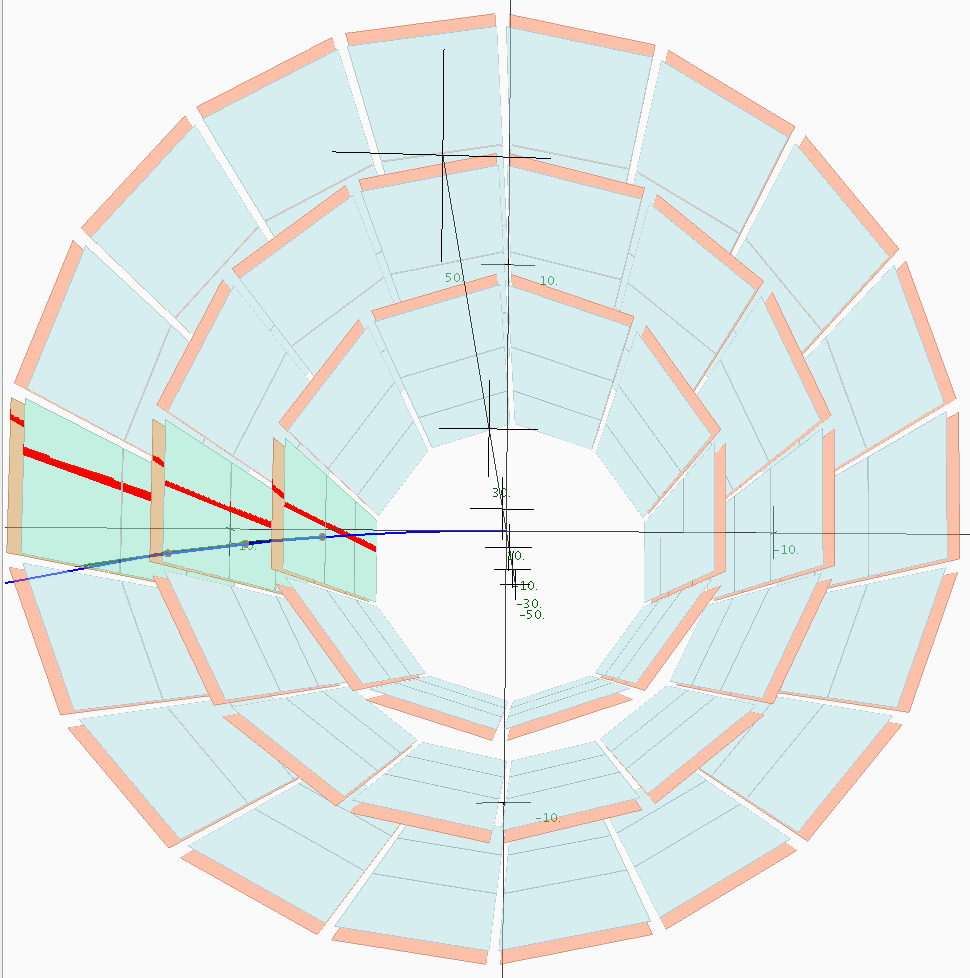
\includegraphics[width=1.0\columnwidth,keepaspectratio]{svt3dview.png}
\caption{3D view of the simulated SVT detector geometry.}
\label{fig:svt3dview}
\end{figure}

According to the results of GEANT simulation of the SVT, a resolution of 50~$\mu$m in the bending plane is needed to measure, with a precision better than 5$\%$, tracks with momentum up to 1~GeV (see Fig.~\ref{fig:PtRes}) \cite{MC1,MC2}. At low momenta the degradation of the resolution is caused by multiple scattering.

\begin{figure}[hbt]
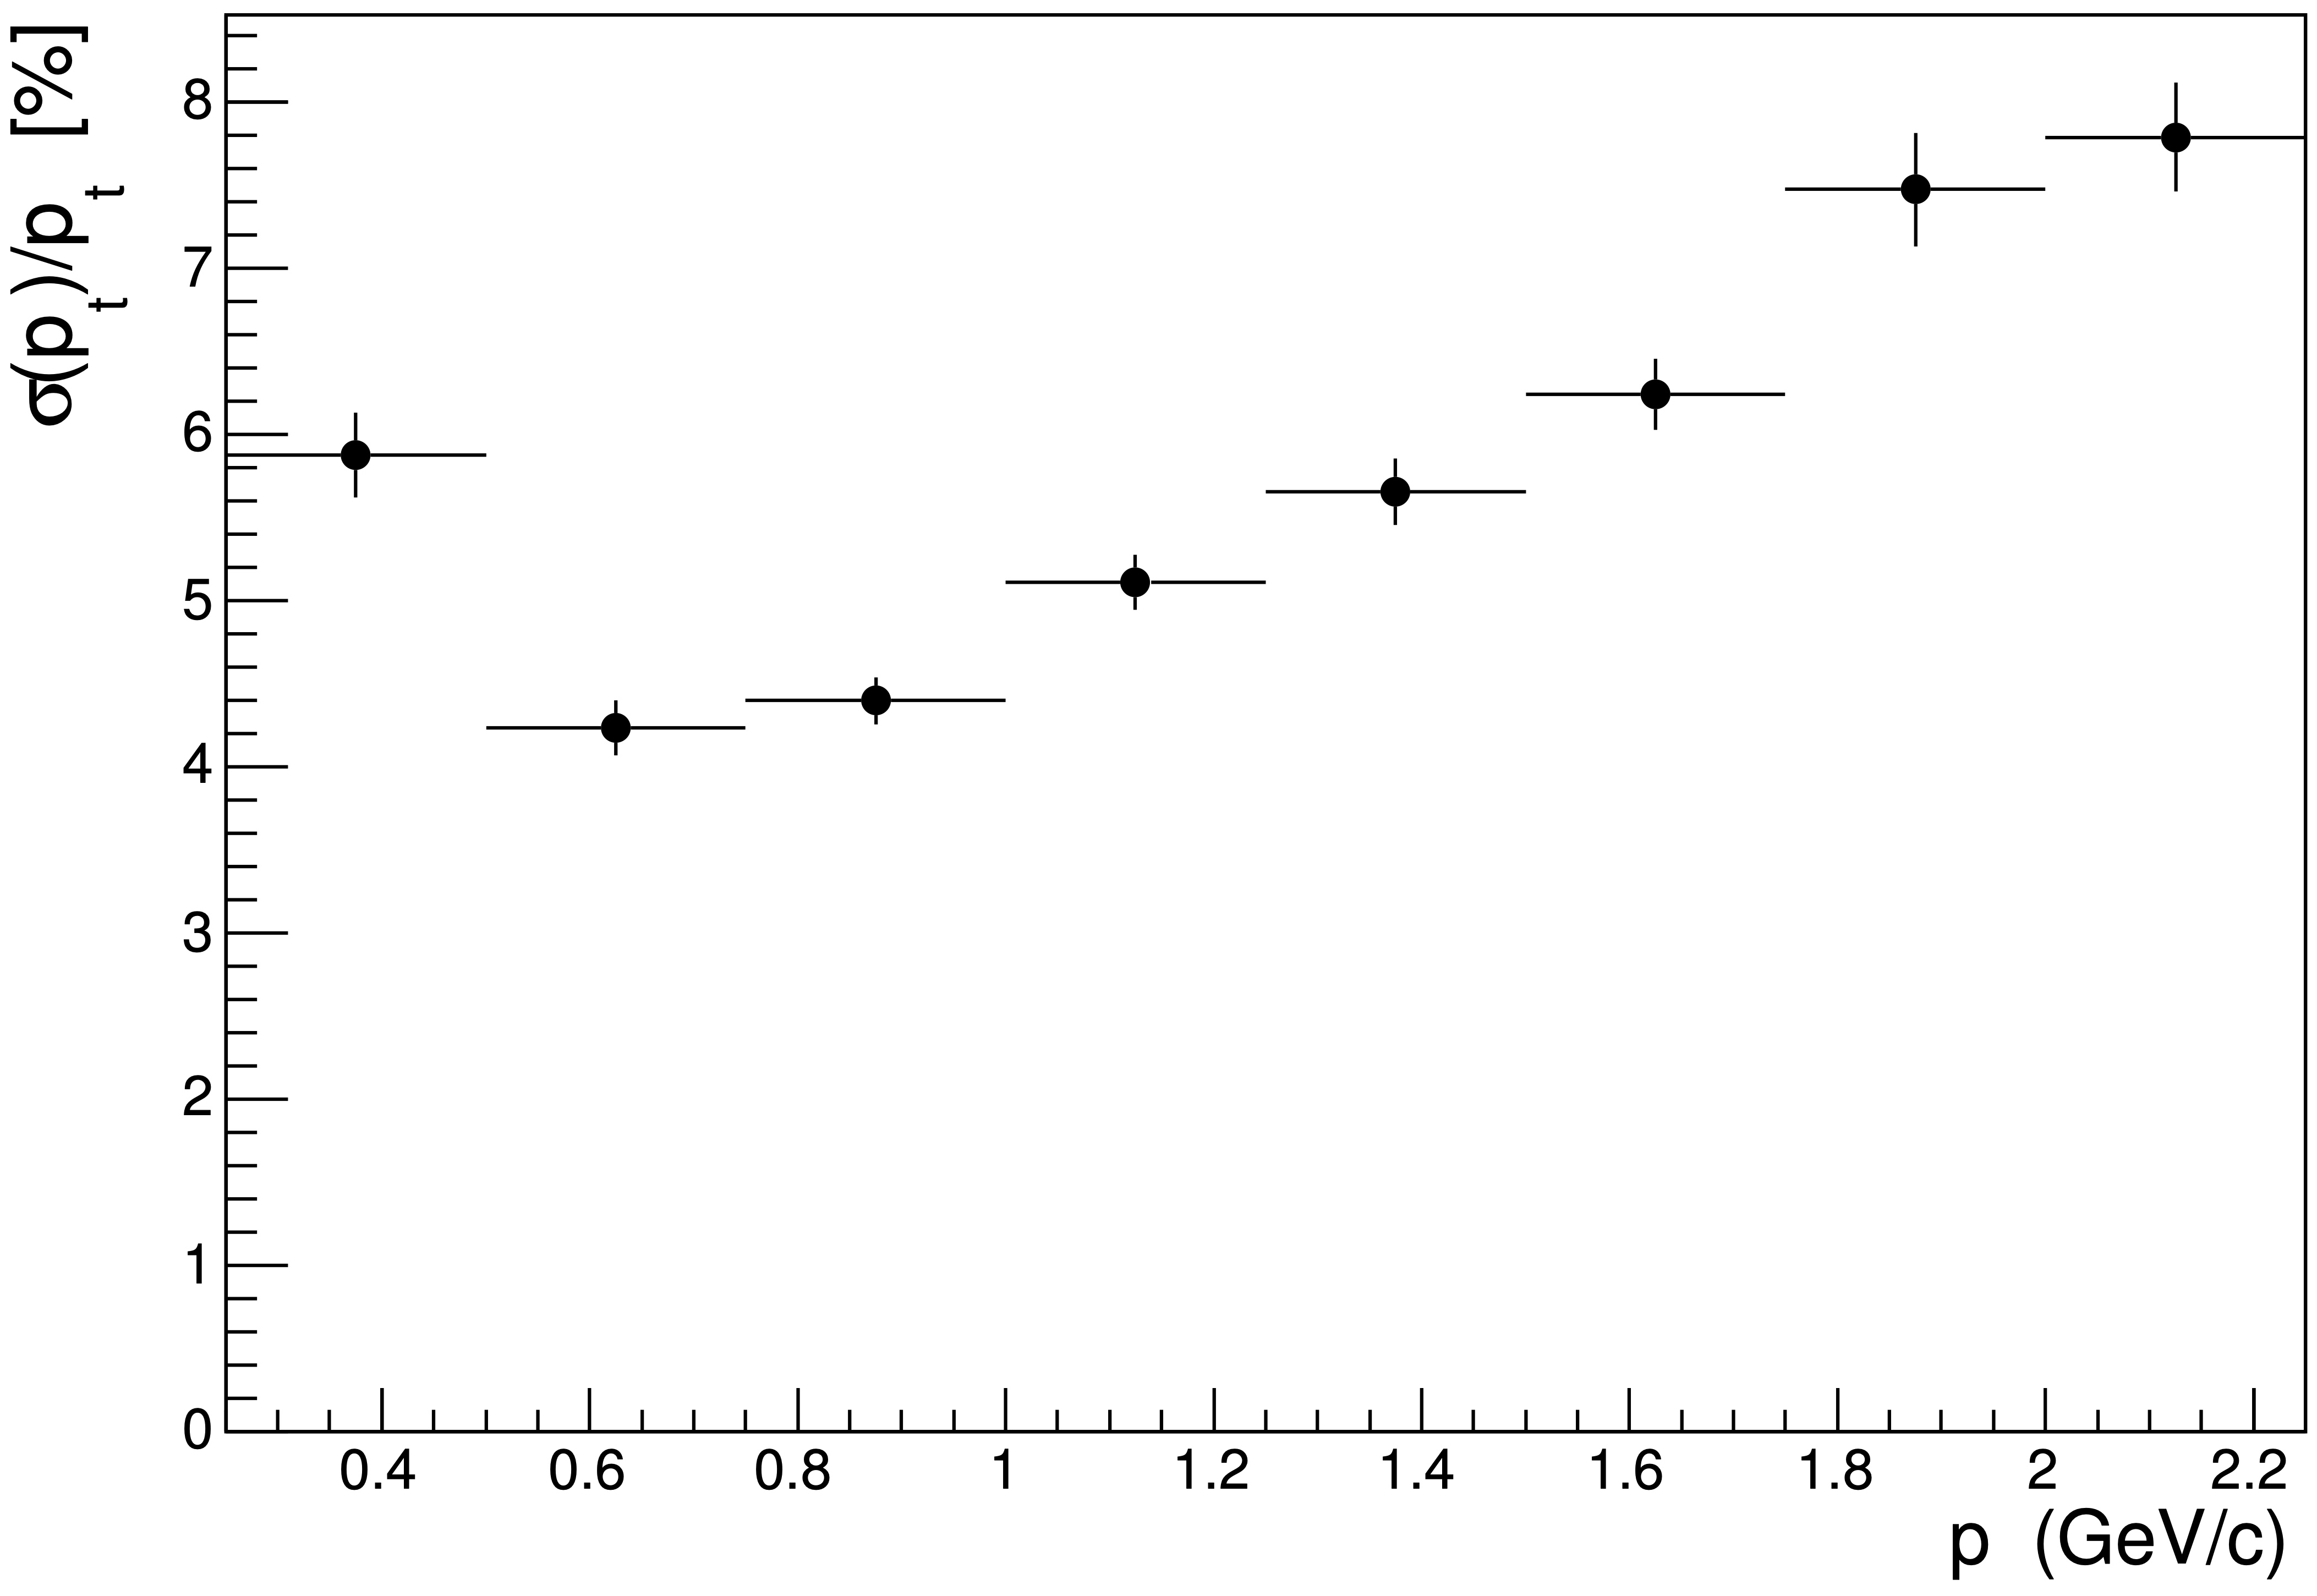
\includegraphics[width=1.0\columnwidth,keepaspectratio]{PtResol.jpg}
\caption{Simulated SVT momentum resolution.}
\label{fig:PtRes}
\end{figure}

The centroid residual distribution for the simulated muon tracks generated in the interval 0.5--2 GeV is shown in Fig.~\ref{fig:centroid-residual-mc}. The cluster centroids were calculated based on the charge weighting method. The spacial resolution of the sensors in the transverse plane using the ideal SVT geometry with no misalignments was found to be about 30~$\mu$m. 

\begin{figure}[hbt]
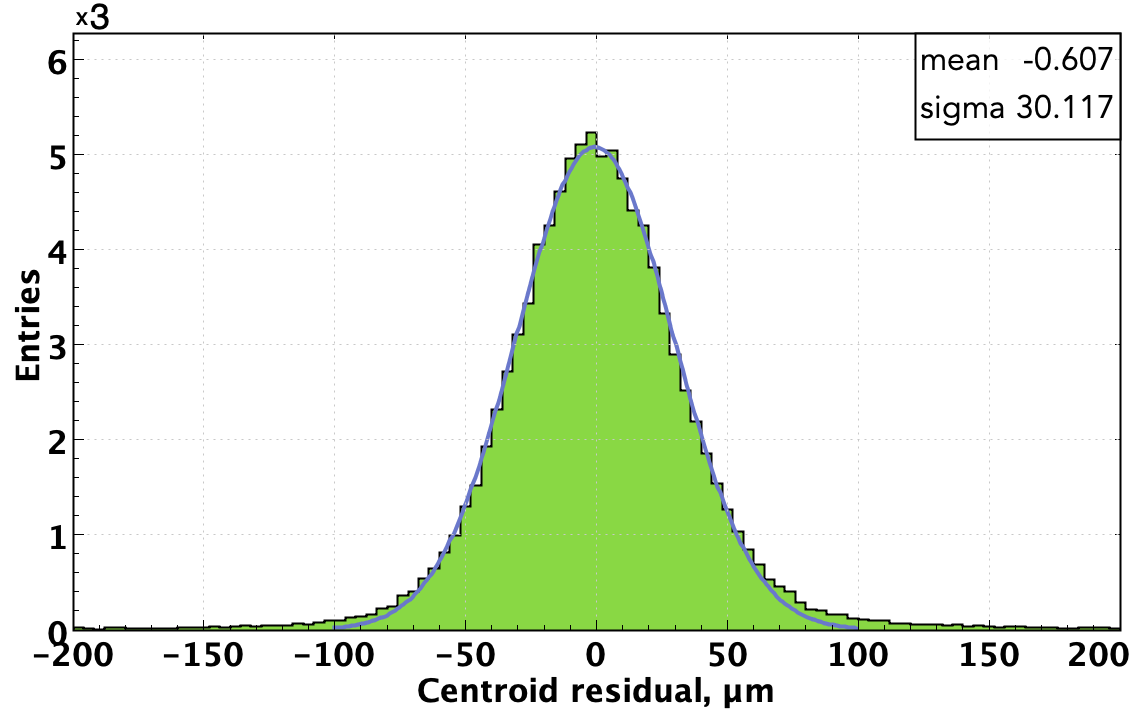
\includegraphics[width=1.0\columnwidth,keepaspectratio]{centroid-residual-mc.png}
\caption{Simulated centroid residual distribution for the SVT module.}
\label{fig:centroid-residual-mc}
\end{figure}

\subsection{Backgrounds, Energy Deposition, Dose Rates}

Radiation-induced bulk and surface detector damage studies have been conducted with charged hadrons, leptons, neutrons, and $\gamma$-ray photons. The damage can be due to ionizing radiation, affecting the surface, and non-ionizing energy loss from the hadrons interacting with the sensors and introducing lattice defects. The new energy levels within the band gap lead to increase of the leakage current, charge trapping, and change of the effective doping concentration. The radiation damage produced by different particles with different energies is scaled under the assumption of the Non-Ionizing Energy Loss (NIEL) hypothesis as the radiation damage in the silicon bulk depends only on the non-ionizing energy loss. The damage caused by different particles is referenced to the damage from 1 MeV neutrons. The standard value for the NIEL of 1 MeV neutrons is 95 MeVmb. 

\begin{figure}[hbt] 
\centering 
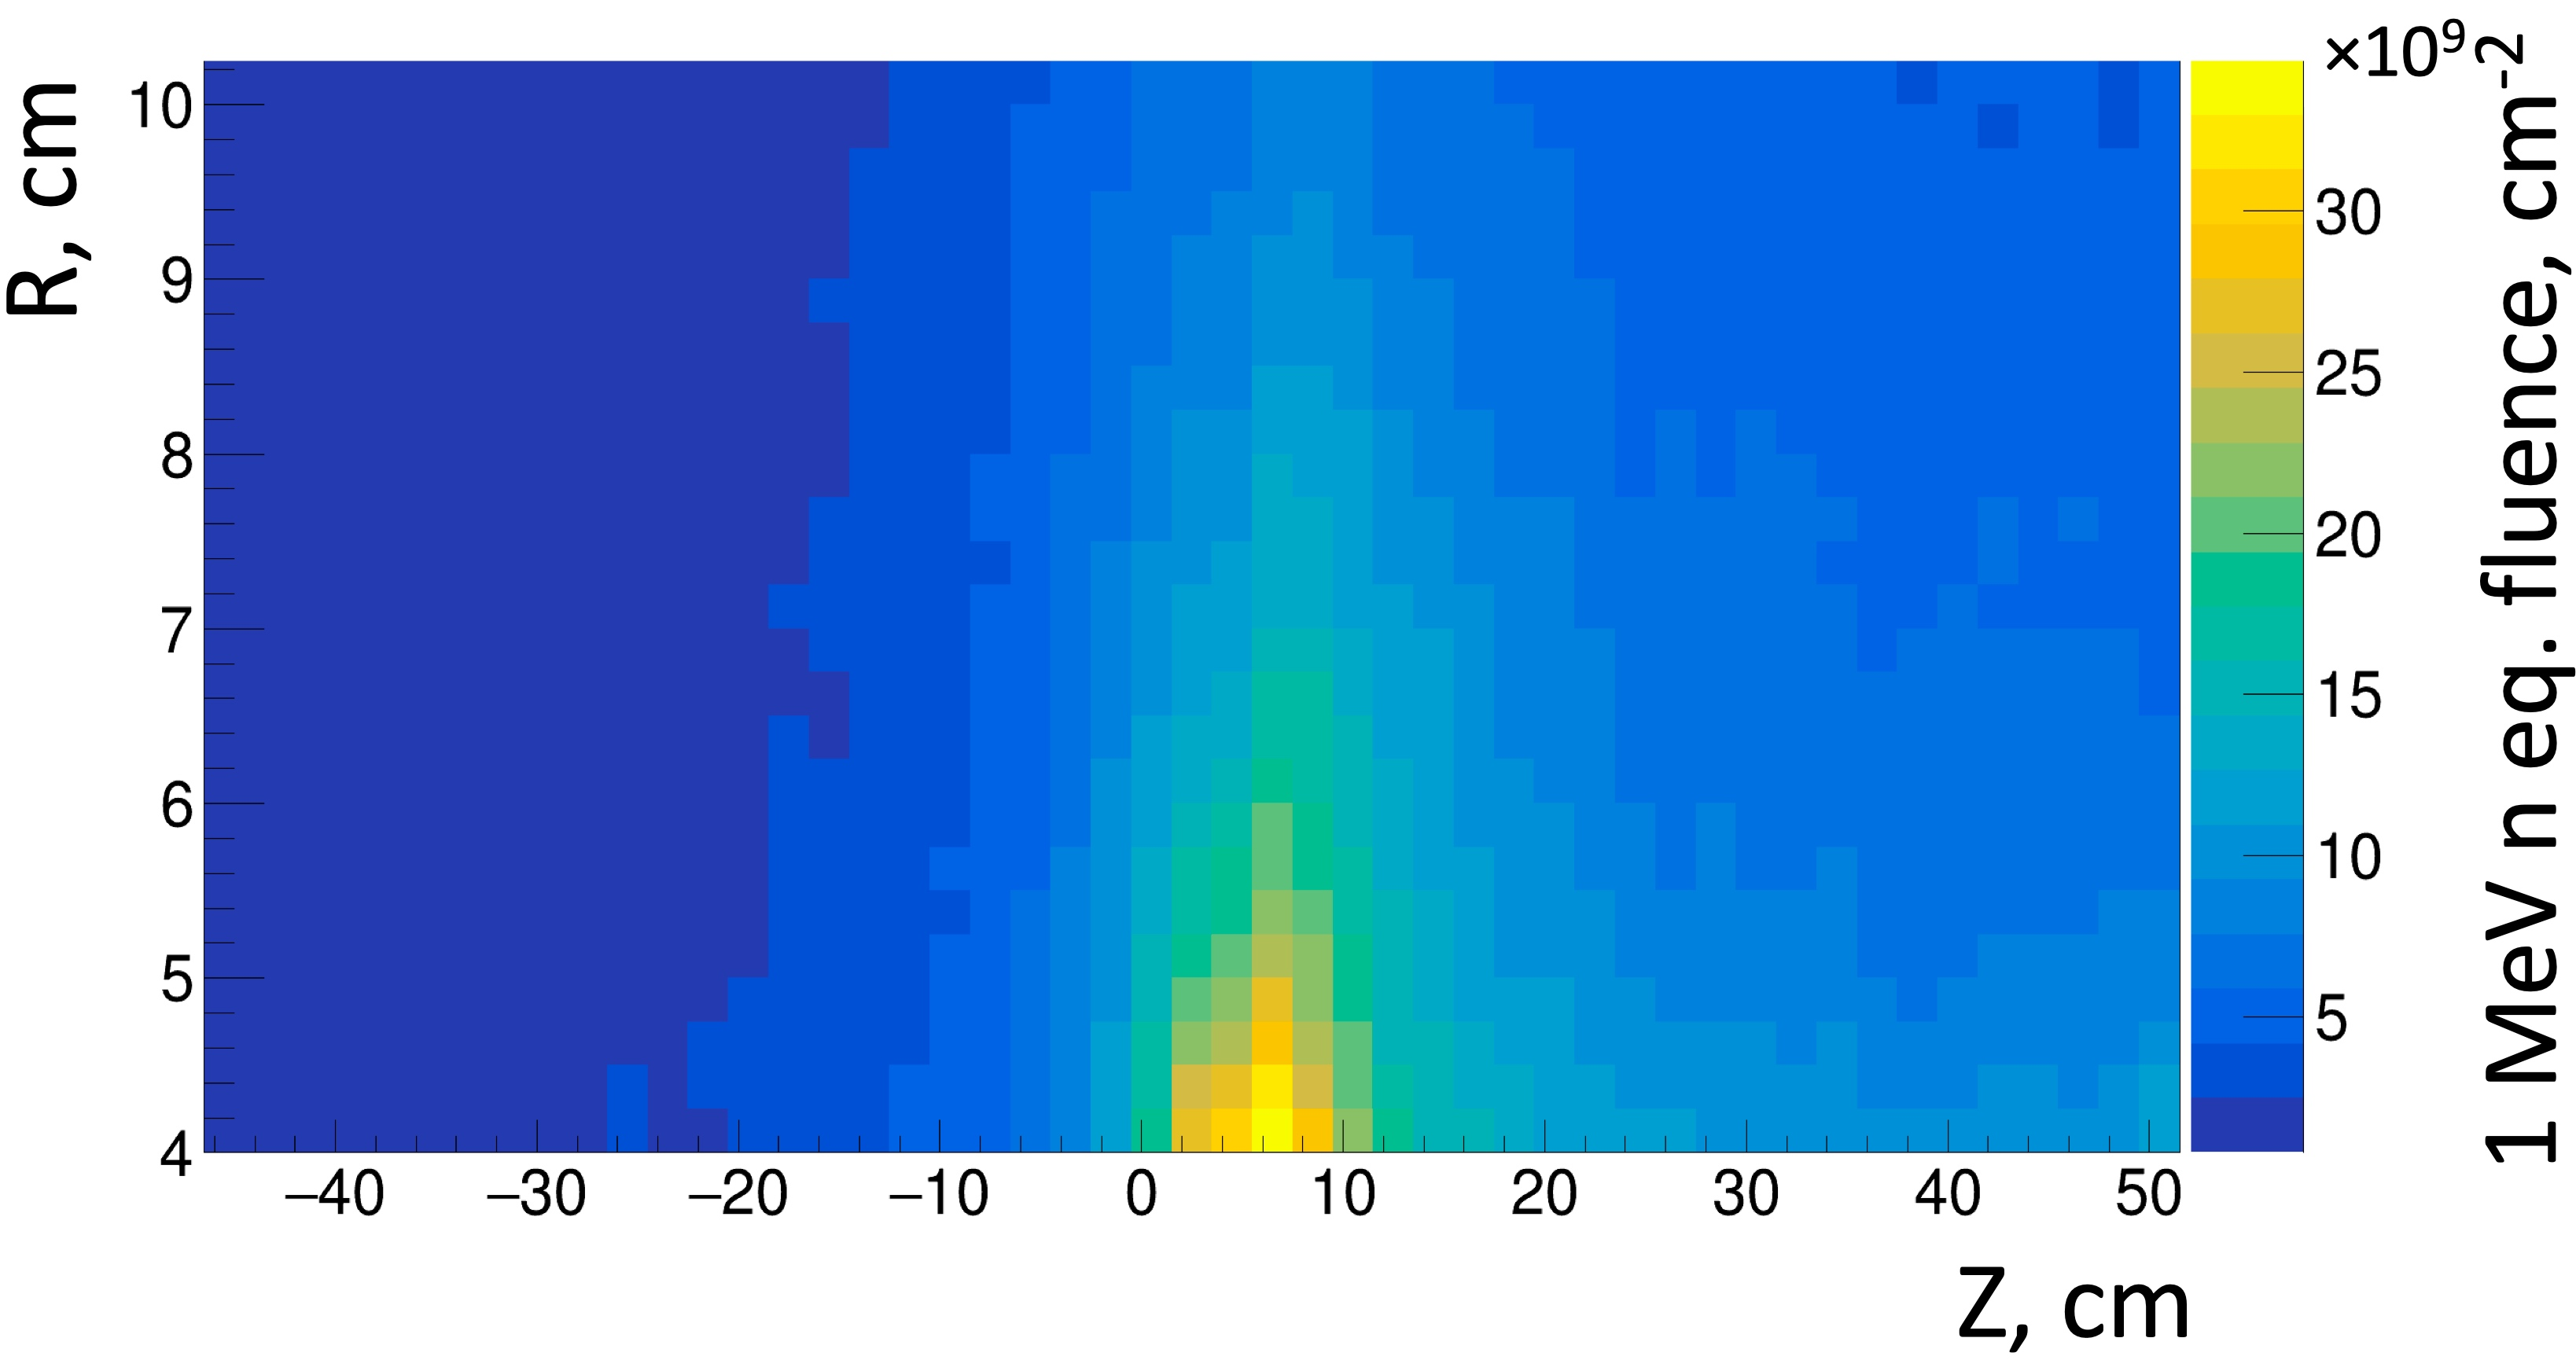
\includegraphics[width=1.0\columnwidth,keepaspectratio]{Pb_1MeVeq.jpg}
\caption{Accumulated 1MeV equivalent neutron fluence for the lead target.}
\label{fig:fluka1}
\end{figure}

To calculate the effects of different target configurations on the SVT detector,  FLUKA~\cite{FLUKA1, FLUKA2} simulations have been performed. In order to include hadron electro-nuclear production, a dedicated source term has been used to enhance the physics production from the target, since it is of key importance in radiation estimates for targets with radiation length below 4$\%$. To assess the radiation damage to the SVT, the accumulated 1~MeV neutron equivalent fluence has been recorded corresponding to the planned run conditions. For the experiment with the lead target, the expected exposure was 240 hours at a beam current of 38~nA with an electron beam energy of 6.6~GeV (see Fig.~\ref{fig:fluka1}). For a deuterium target, the study has been done for the accumulated charge of 108 mC at 11 GeV (see Fig.~\ref{fig:fluka2}). In both scenarios the expected doses should not cause substantial degradation of the silicon sensors.

\begin{figure}[hbt] 
\centering 
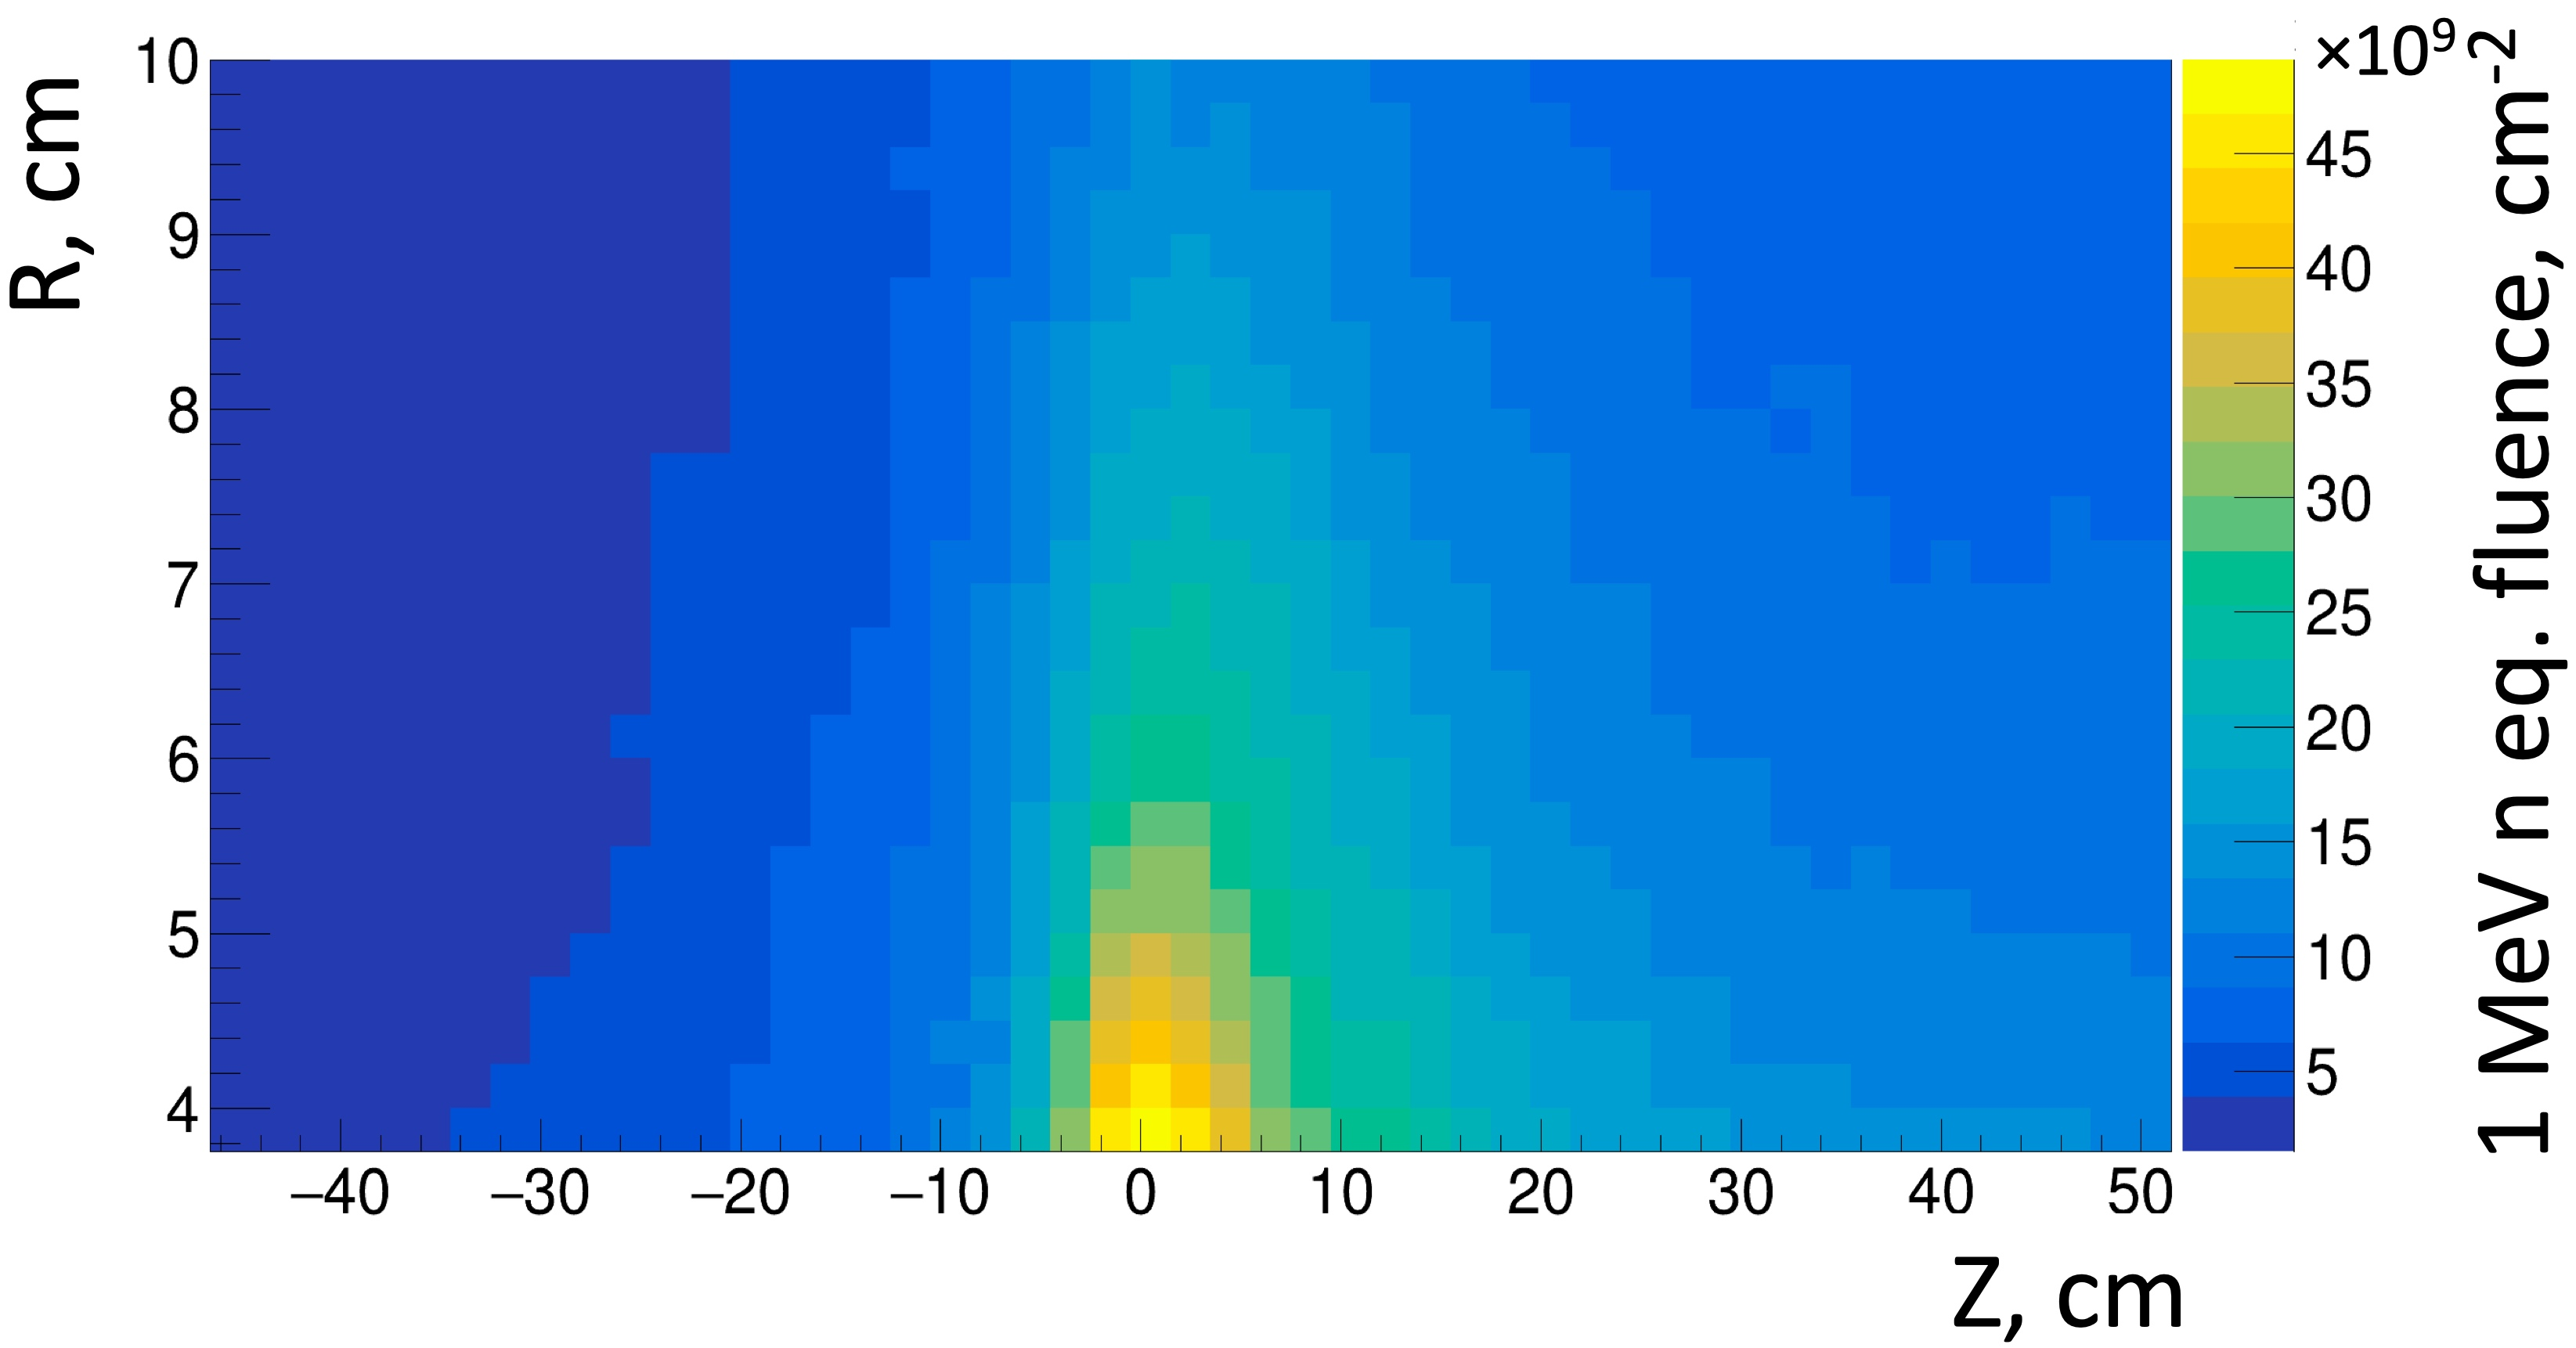
\includegraphics[width=1.0\columnwidth,keepaspectratio]{Deuterium_1MeVeq.jpg}
\caption{Accumulated 1MeV equivalent neutron fluence for the deuterium target.}
\label{fig:fluka2}
\end{figure}

FLUKA simulations of radiation damage levels have been performed in terms of 1~MeV equivalent neutron fluence and high energy hadron equivalent fluence that is proportional to the rate of Single Event Effects (SEE)~\cite{FLUKA3}. Estimated levels of radiation damage in the radial direction are presented in Fig.~\ref{fig:rad-levels-radial} for liquid hydrogen and carbon targets at nominal beam currents. Also shown are the radiation levels for the tagger magnet yoke during the beam tuning~\cite{BEAMLINENIM}.

\begin{figure}[hbt] 
\centering 
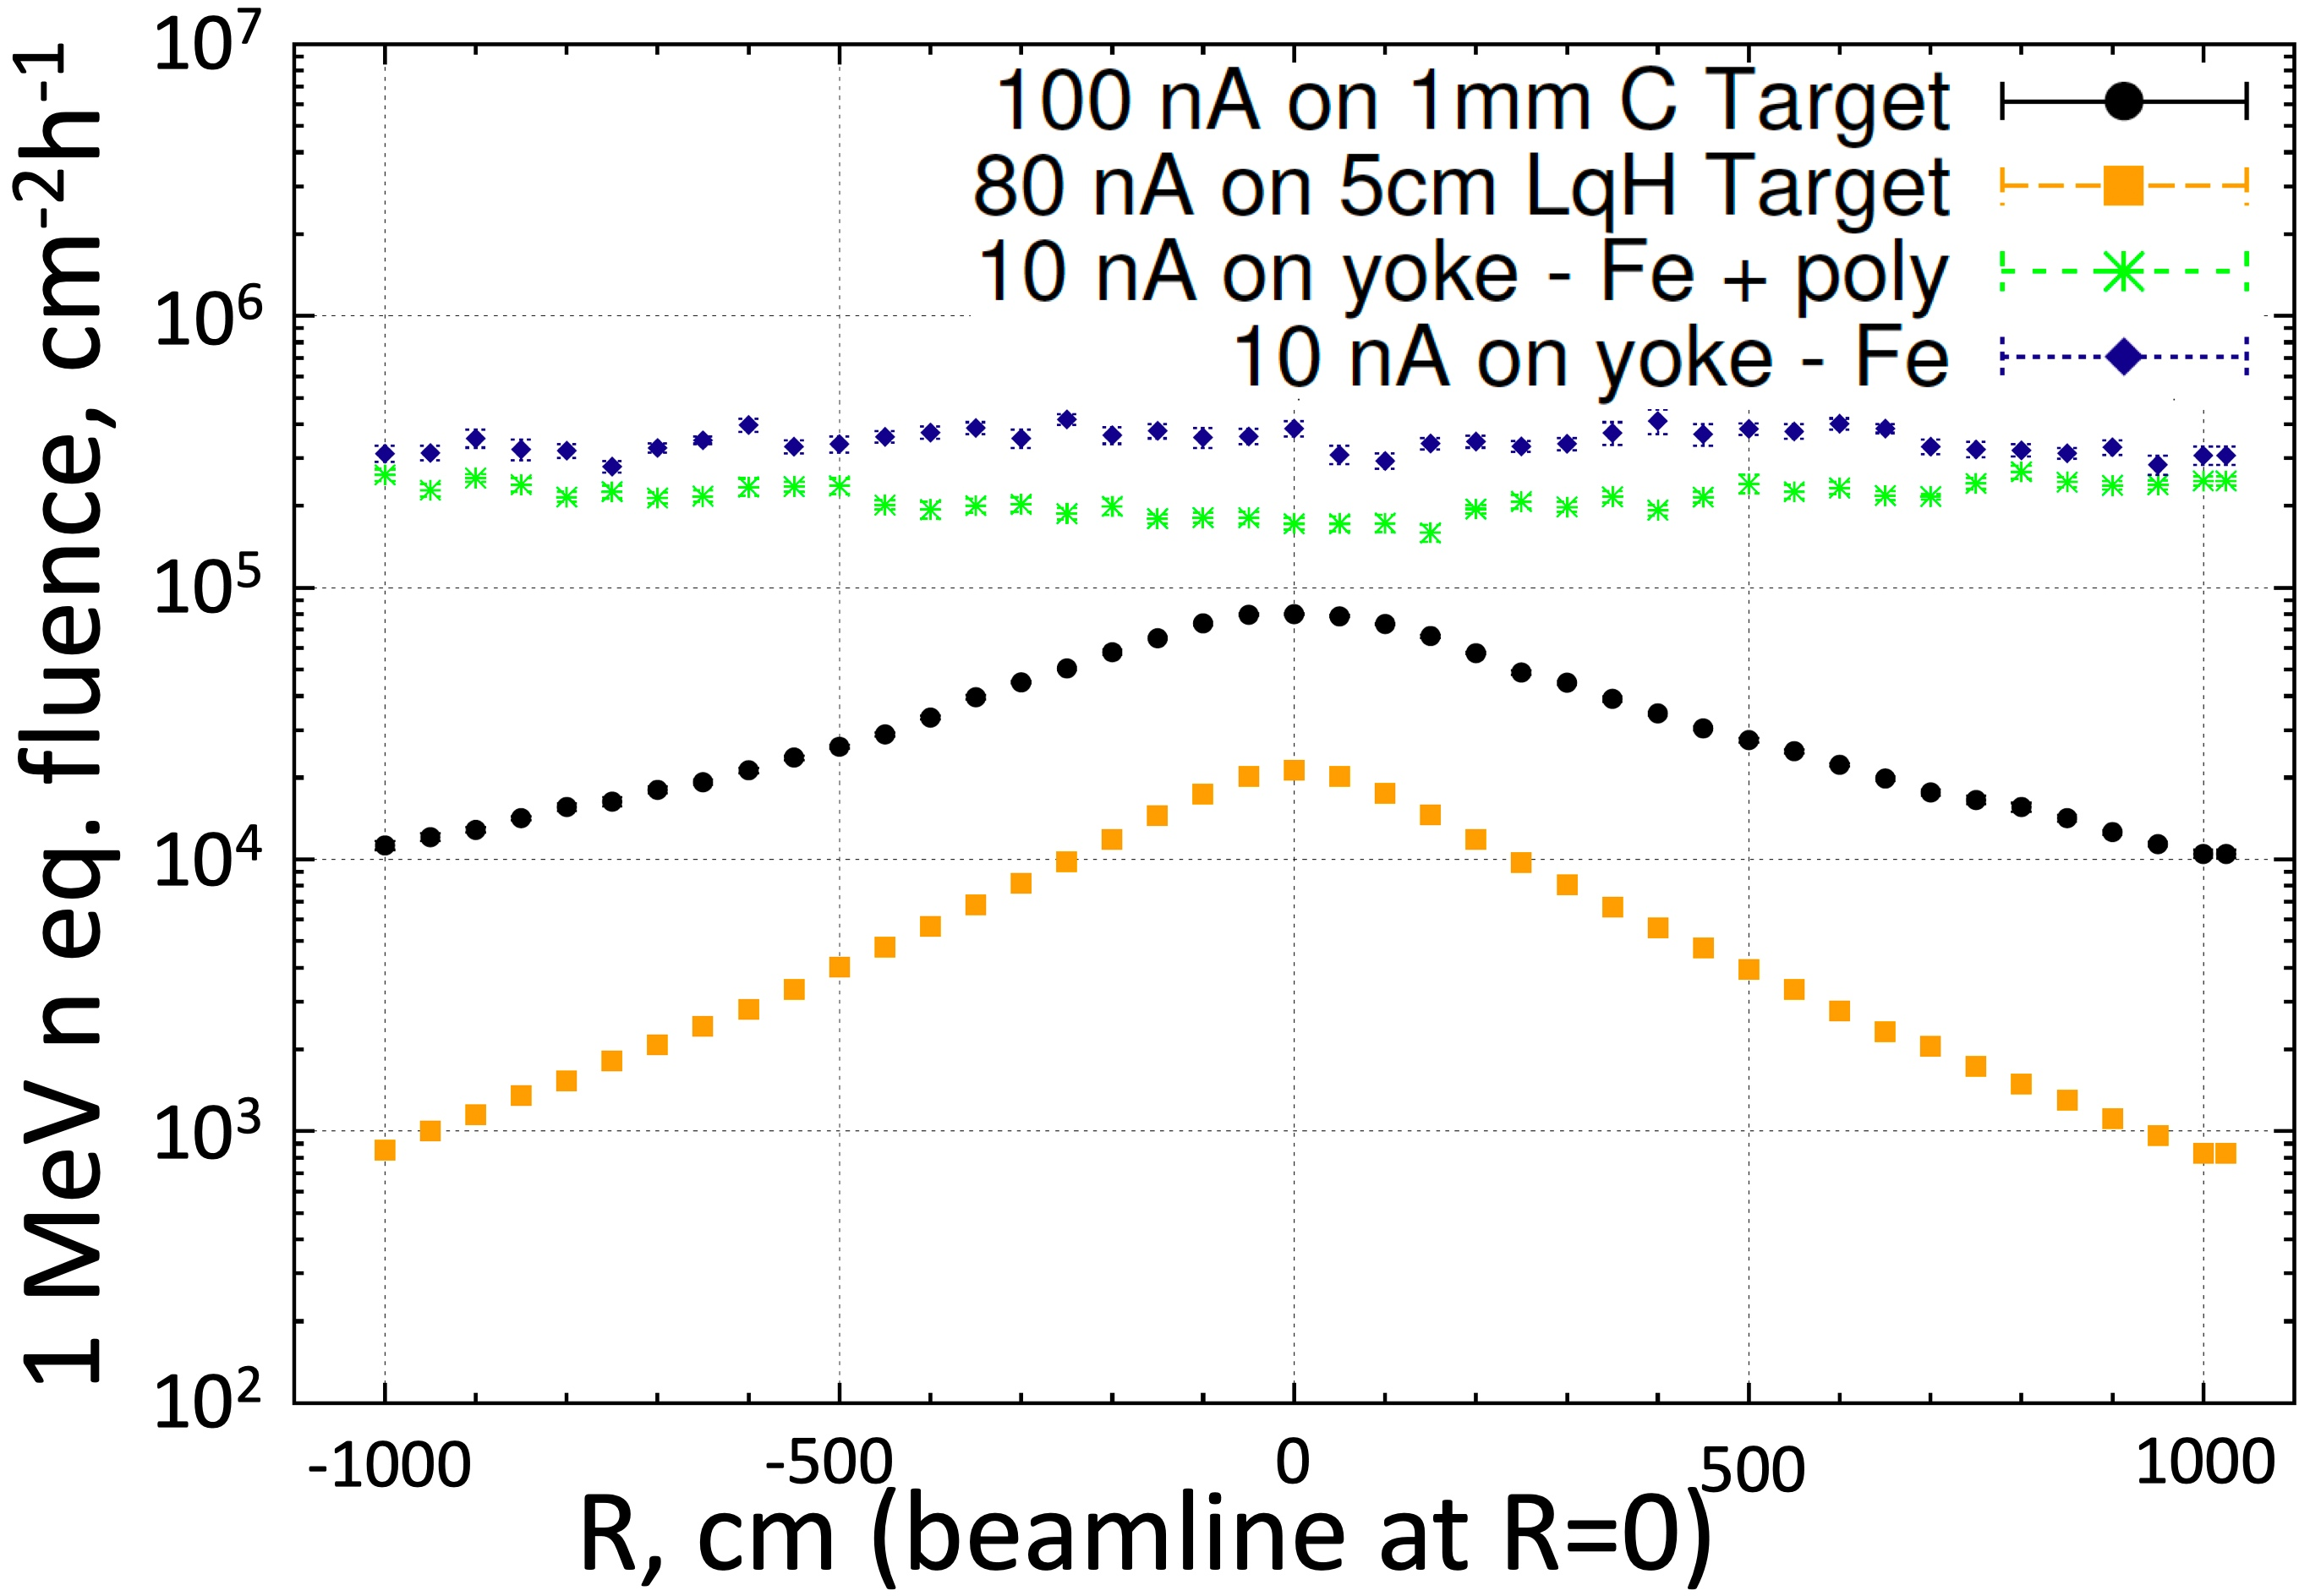
\includegraphics[width=1.0\columnwidth,keepaspectratio]{rad-levels-radial.jpg}
\caption{Estimated levels of radiation damage in radial direction in terms of 1MeV neutron equivalent fluence in silicon.}
\label{fig:rad-levels-radial}
\end{figure}
 
\begin{figure}[hbt] 
\centering 
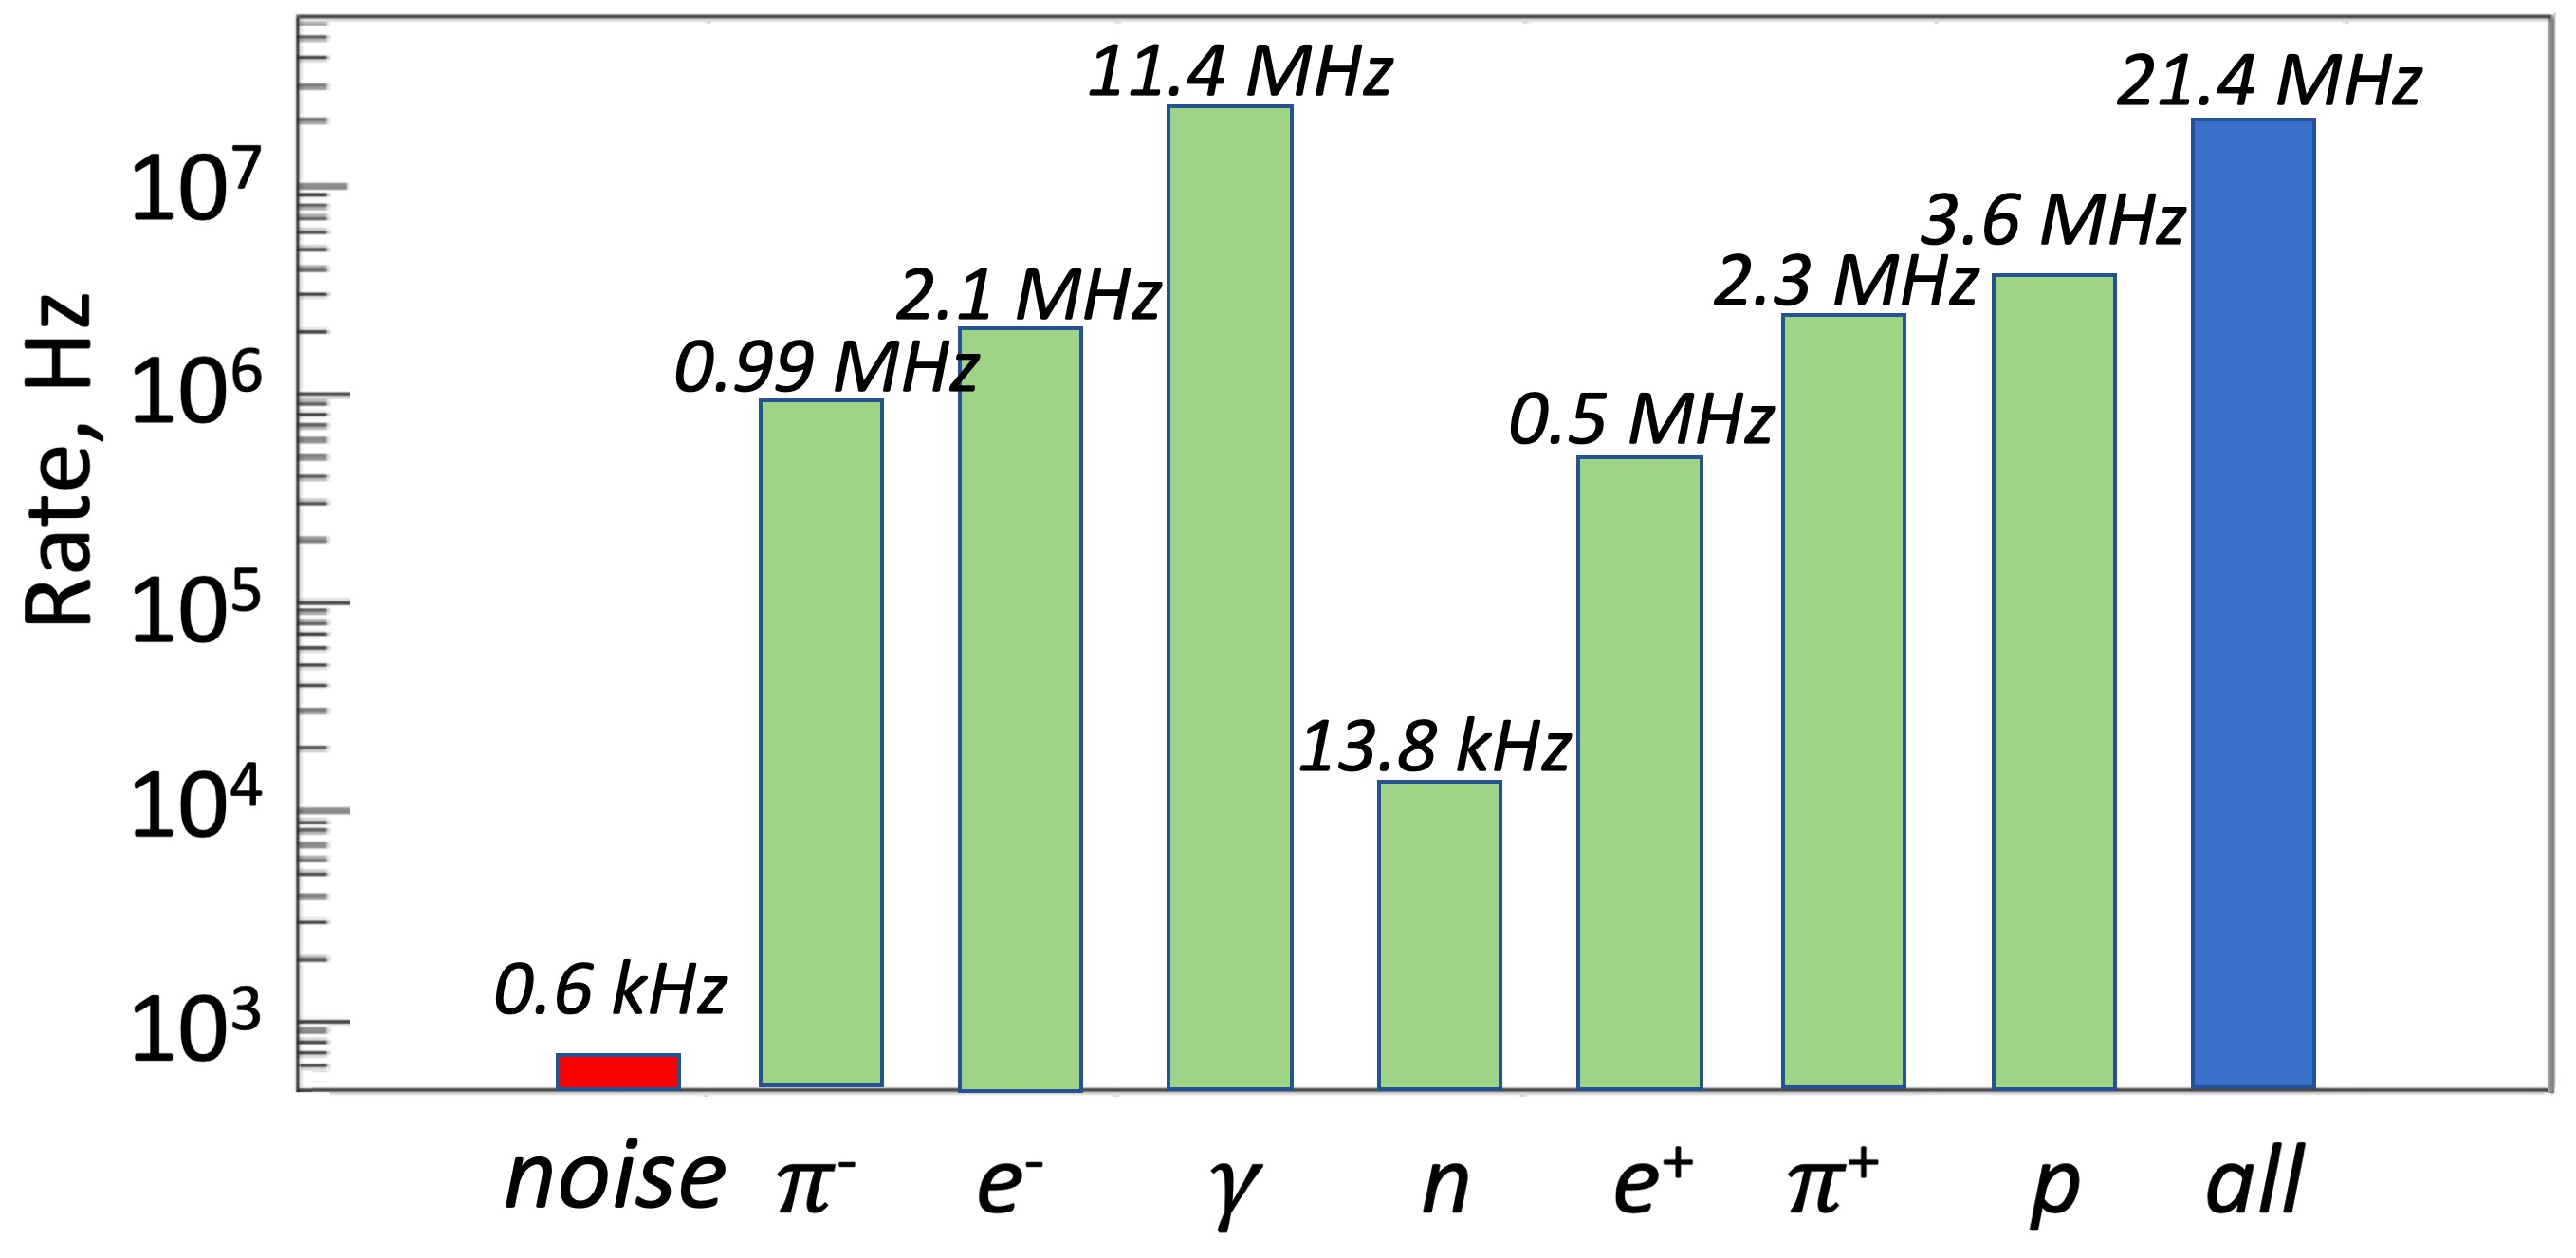
\includegraphics[width=1.0\columnwidth,keepaspectratio]{rates-lh2.jpg}
\caption{Rates in the first SVT layer for a 5-cm long liquid hydrogen target at the nominal CLAS12 operating luminosity of 10$^{35}$cm$^{-2}$s$^{-1}$.}
\label{fig:rates-lh2}
\end{figure}

Geant 4-based calculations of fluences, radiation doses, and 1 MeV neutron damage rates in the SVT were performed for different particles using CLAS12 GEMC (see simulations section in this volume). The SVT rates were estimated for liquid hydrogen, liquid deuterium, carbon, iron, and lead targets. For each event, 124,000 electrons going through the target within a 248.5-ns time window were simulated. This corresponds to the full CLAS12 10$^{35}$cm$^{-2}$s$^{-1}$ luminosity on a 5-cm-long liquid-hydrogen target at 11 GeV beam energy. Rates in the first SVT layer for a 5-cm thick liquid-hydrogen target are shown in Fig.~\ref{fig:rates-lh2}. For a carbon target at a threshold of 40 keV the hadronic rate was estimated to be 5 MHz (total rate 40 MHz) with strip hit rates of 3.1 kHz (Region 1), 2.2 kHz (Region 2), and 1.7 kHz (Region 3). The energy deposited in layer 1 for the electromagnetic and the hadronic particles is shown in Fig.~\ref{fig:energy-deposited-l1}. At a threshold of 30 keV, 92$\%$ of the electromagnetic background is rejected while preserving  99.5$\%$ of the signals coming from the hadrons~\cite{TDRSVT}.

\begin{figure}[hbt] 
\centering 
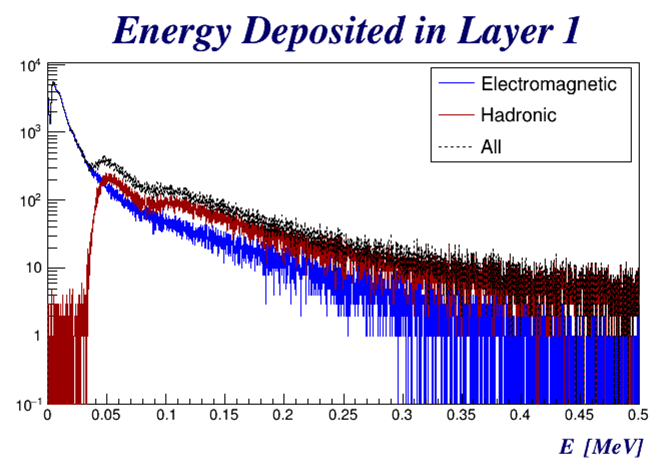
\includegraphics[width=1.0\columnwidth,keepaspectratio]{energy-deposited-l1.png}
\caption{Energy deposited in the SVT layer 1 for electromagnetic and hadronic particles for a liquid hydrogen target at the nominal CLAS12 operating luminosity.}
\label{fig:energy-deposited-l1}
\end{figure}

Simulations of beam-related backgrounds were performed for several thicknesses of a tungsten shielding cylinder around the CLAS12 target covering the first SVT layer. A tungsten shield 51~$\mu$m thick is installed on the target scattering chamber. The shield consists of 2 sheets mounted over the top and bottom halves of the foam cylinder referenced to the SVT common ground. The SVT rates and radiation damage benefit from the inclusion of the tungsten shield. The rates have been compared with physics run data at several beam currents.

While the gamma fluences / doses show a dramatic decrease with the introduction of shielding, the total fluences and doses decrease significantly for the thinner configuration and do not vary much for thicker tungsten (see Fig.~\ref{fig:rates-l1}). The photon radiation dose becomes negligible for 50 $\mu$m or more of tungsten with total 1 MeV equivalent radiation dose about 65 krad per year on a liquid-hydrogen target. For 15 years of running the experiment on a carbon target the estimated radiation dose for the sensors is 2.5~Mrad (with 50 $\%$ operation) \cite{TDRSVT}. 

\begin{figure}[hbt] 
\centering 
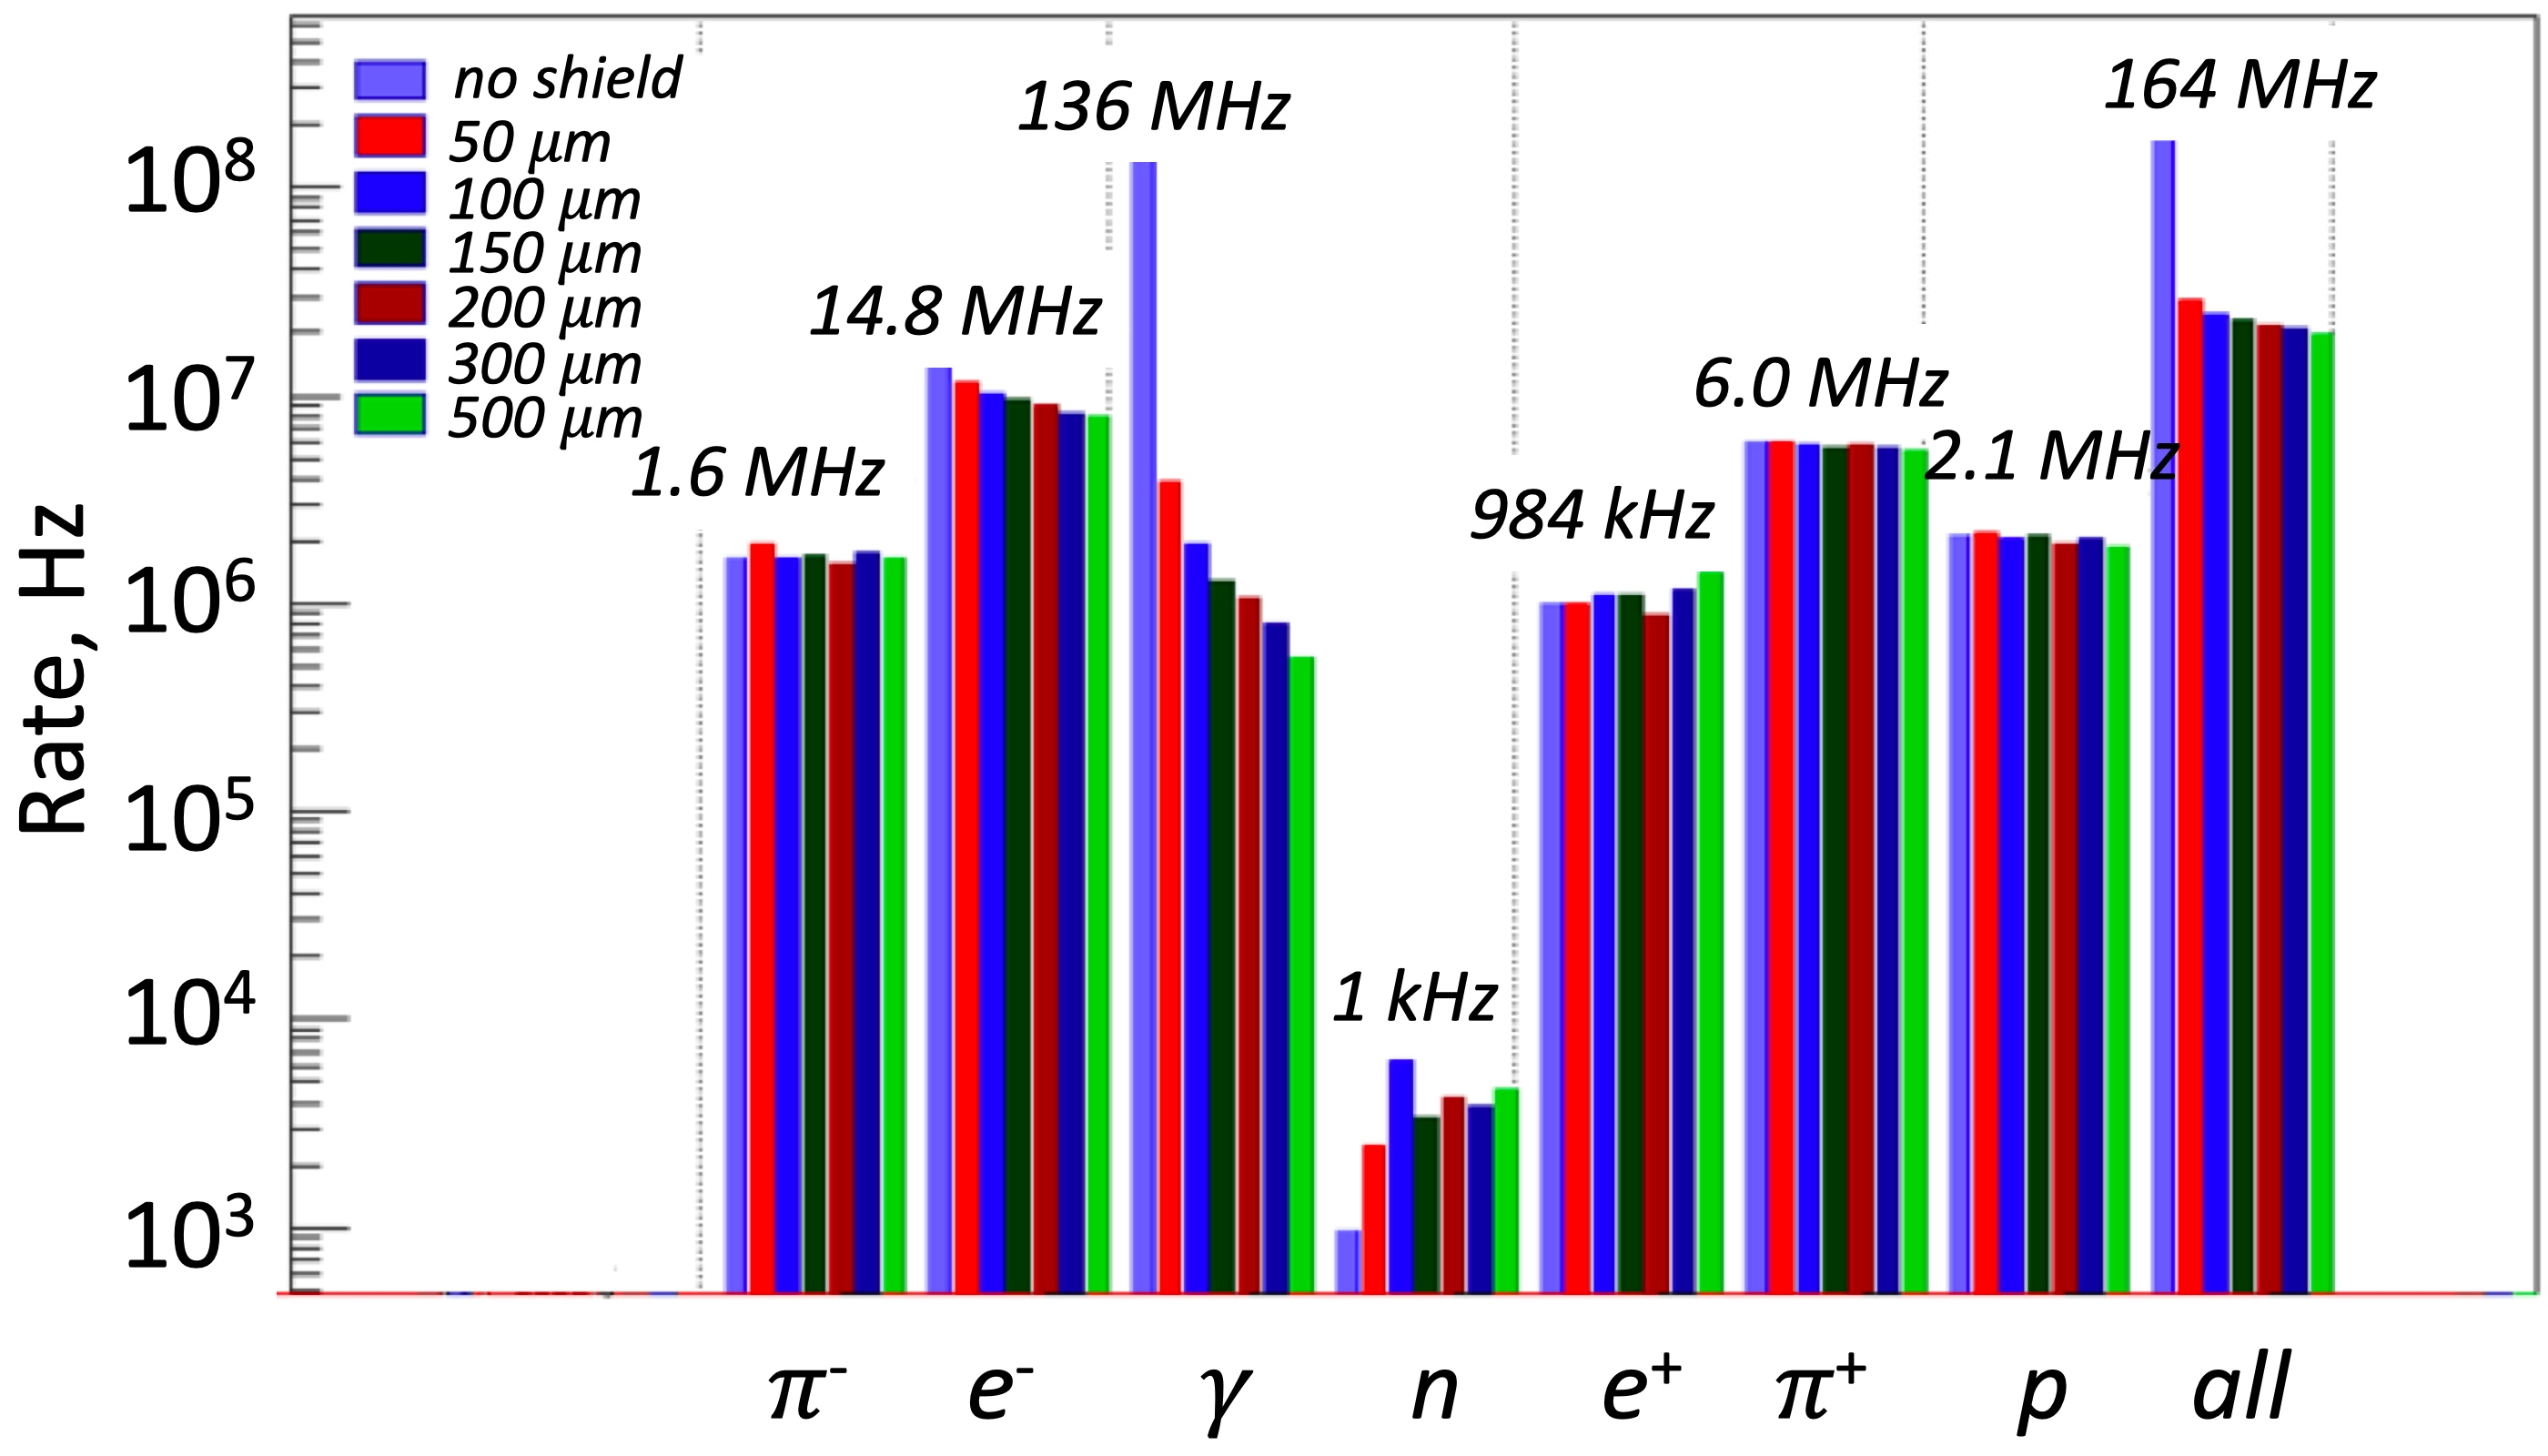
\includegraphics[width=1.0\columnwidth,keepaspectratio]{rates-l1.jpg}
\caption{Rates in the first SVT layer for different tungsten shield thickness from 50 to 500 $\mu$m for a liquid hydrogen target at the nominal CLAS12 operating luminosity. No energy threshold cut applied.}
\label{fig:rates-l1}
\end{figure}

An estimate of the double hit rate from background was performed. Figure~\ref{fig:double-hit-rate} shows the probability of the double hits in the inner region of the SVT. The double hits are the two hits on both sides of a module which are close enough in space to be reconstructed as a cross. The ratio of the double hits to the single hits was found to be about 1$\%$.

\begin{figure}[hbt] 
\centering 
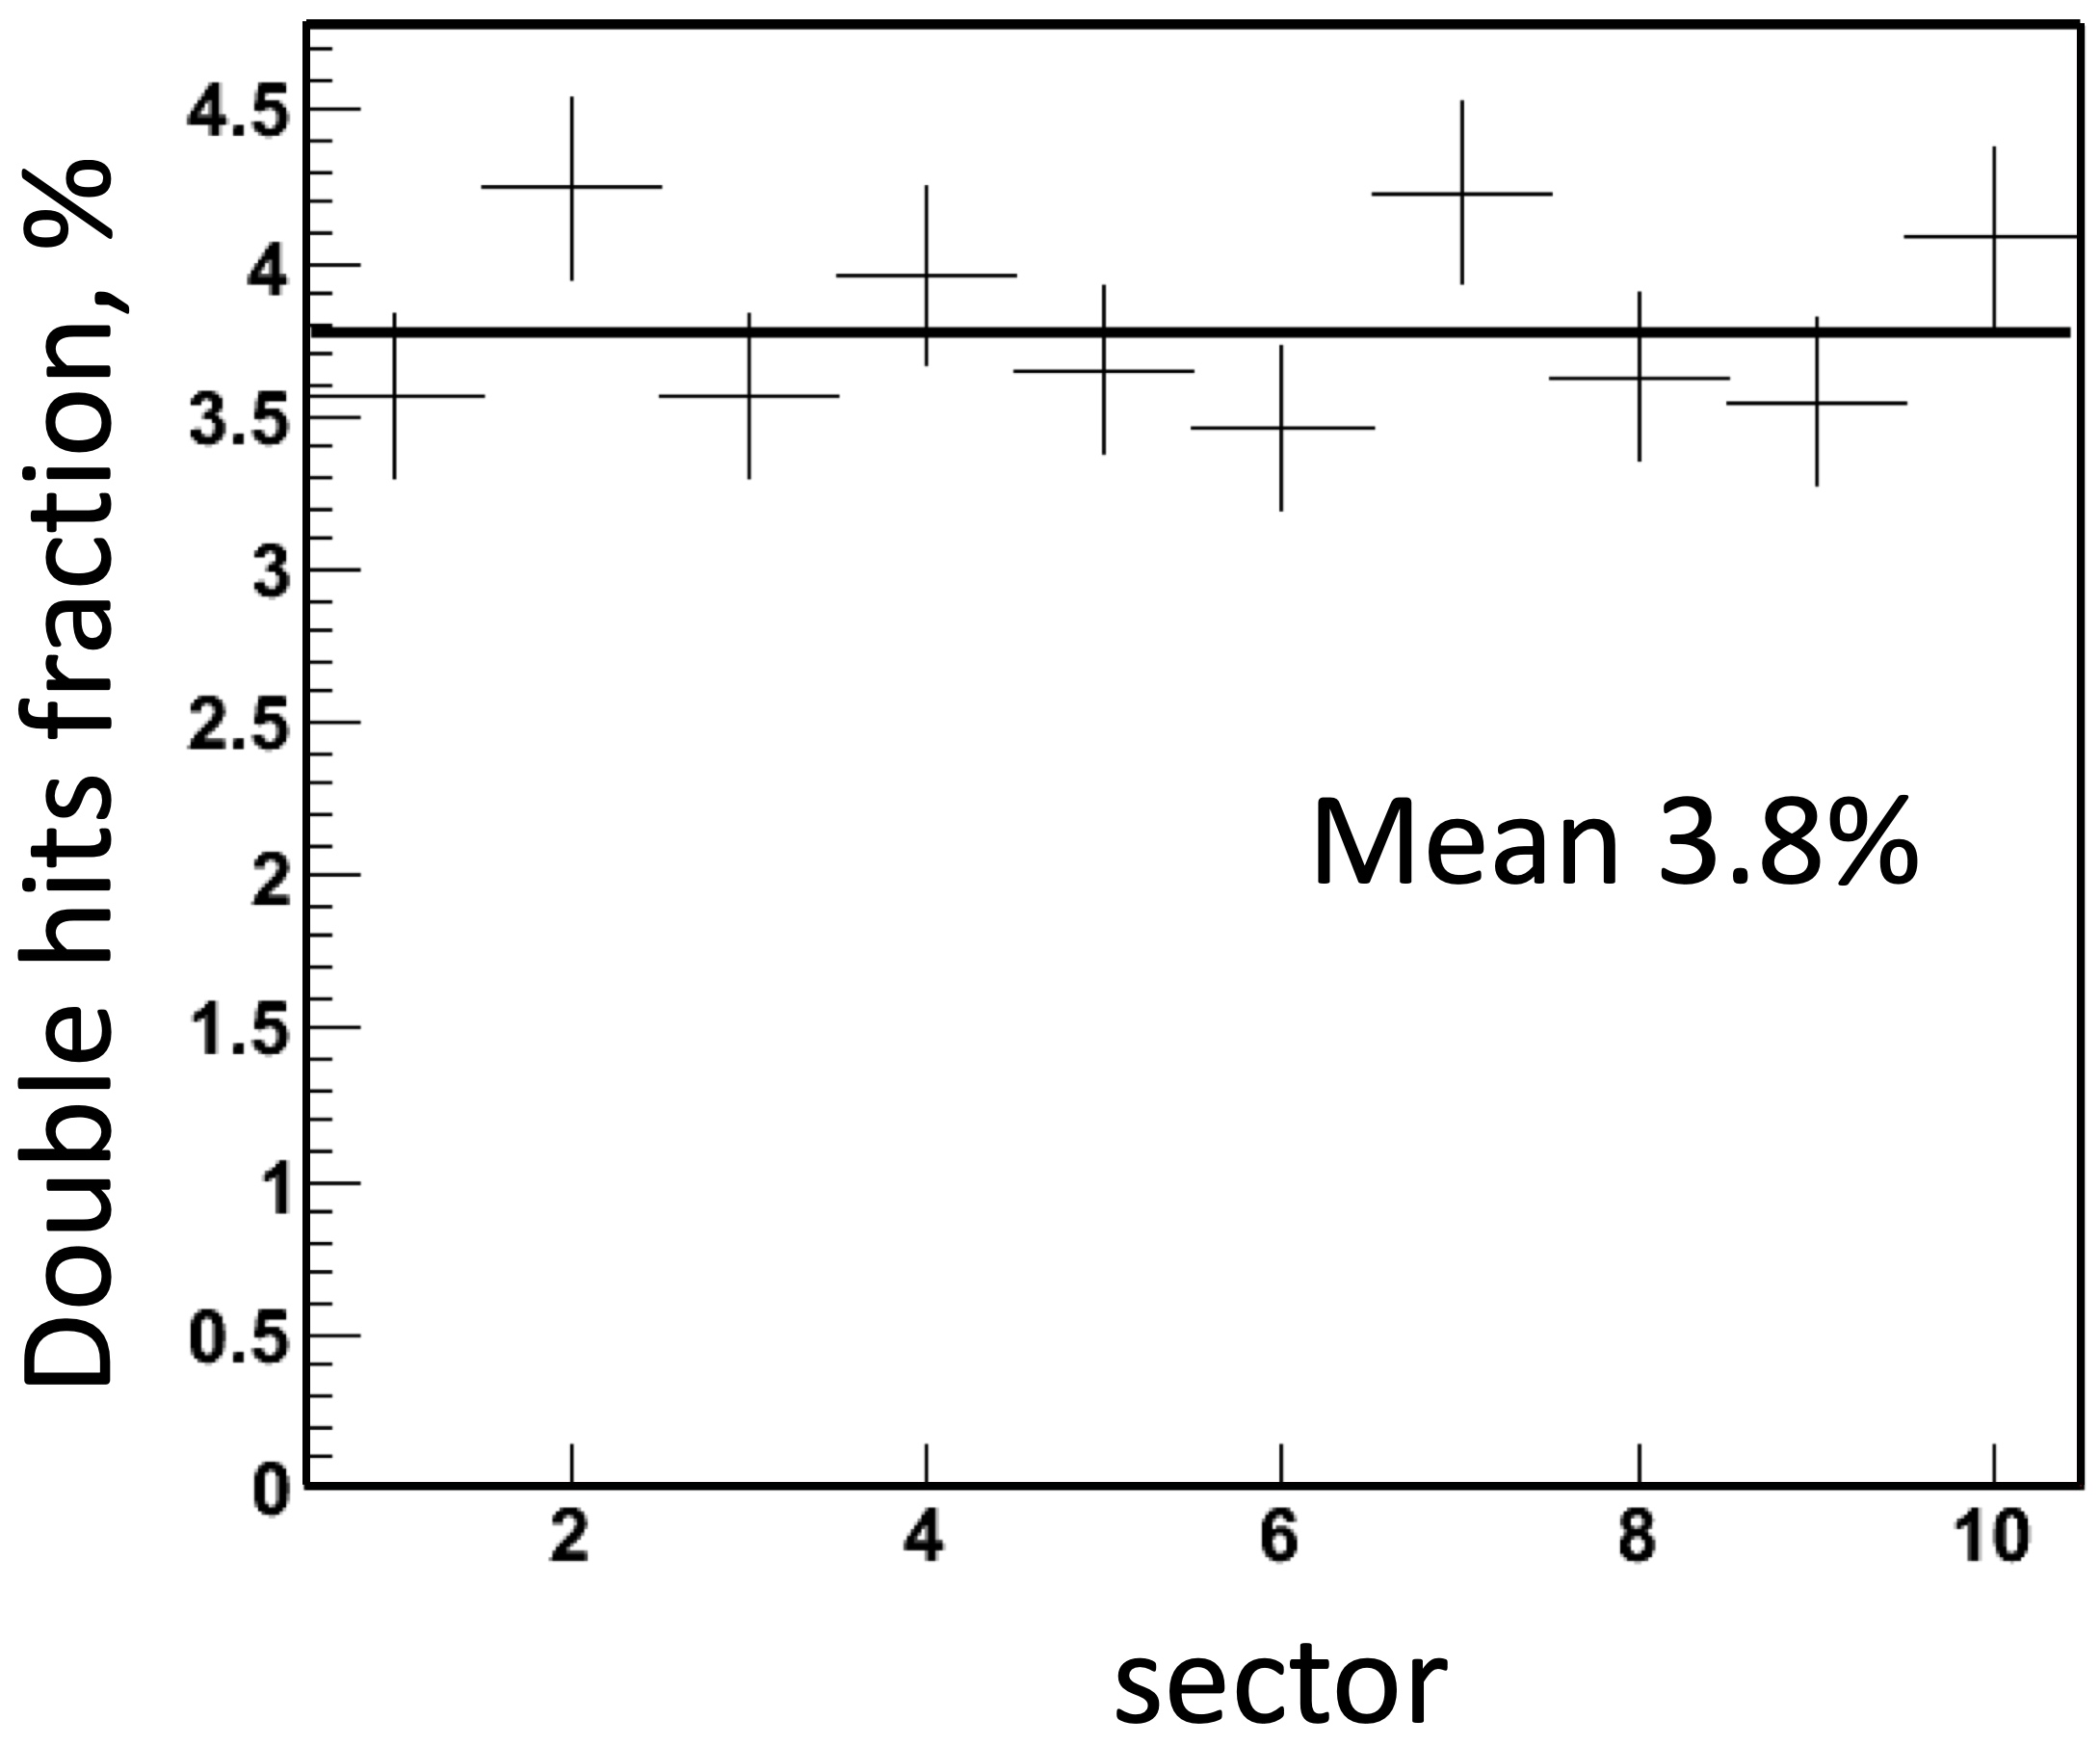
\includegraphics[width=1.0\columnwidth,keepaspectratio]{double-hit-rate.jpg}
\caption{Double hit fraction in Region 1 with the 5-cm long liquid-hydrogen target.}
\label{fig:double-hit-rate}
\end{figure}

\subsection{Magnetic Field}

Due to the constraints on the maximum length of the cables, the readout, slow controls, and power supply crates are installed on a movable service cart within few meters from the detector. To assess the potential impact of the solenoid field on the SVT DAQ, a magnetic field map was simulated for the location of the power supply and readout crates. Figure~\ref{fig:solenoid-field} shows that the maximum strength of the field for the crates is at an acceptable level of 100 G.

\begin{figure}[hbt] 
\centering 
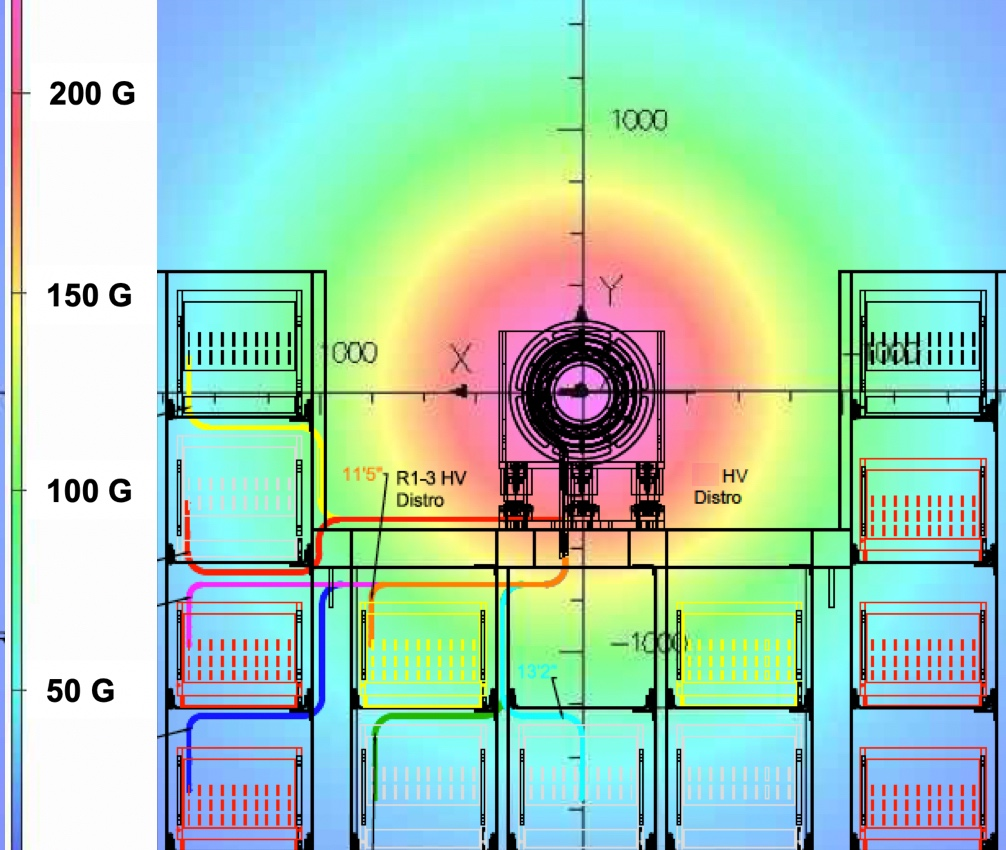
\includegraphics[width=1.0\columnwidth,keepaspectratio]{solenoid-field.jpg}
\caption{Solenoid field map at the location of the SVT service cart.}
\label{fig:solenoid-field}
\end{figure}



